\section{Preliminary Analyses}


We first analyse the potential factors that may affect the tourism industry in Juneau, thus enabling
 a smoother transition to the model building process.

 \subsection{Number of Tourists}

 We found no existing data on the number of tourists visiting Juneau each year, but we can infer it
 by other means.

 According to [1] and [2], among all the transportation methods, cruise ships are the most popular way to visit Juneau,
 accounting for over 90\% of the total number of tourists. As the number of cruise ship passengers is available online, 
 we can use it as a proxy to estimate the total number of tourists.

According to [3], the number of cruise ship passengers visiting Juneau is as follows:

 \begin{table}[H]
    \centering
    \renewcommand{\arraystretch}{1.3}
    \caption{Number of Cruise Ship Visitors to Juneau}
 \begin{tabular}{|c|c|c|c|c|c|c|c|c|c|c|}
    \hline \textit{Year} & 2014 & 2015 & 2016 & 2017 & 2018 & 2019 & 2020 & 2021 & 2022 & 2023 \\
    \hline \begin{tabular}{l} 
    \textit{Num(in thousands)} 
    \end{tabular} & 961 & 983 & 1015 & 1072 & 1151 & 1306 & 0 & 117 & 1167 & 1670 \\
    \hline
    \end{tabular}
\end{table}
It can be easily noted that numbers plummeted in 2020 and 2021 due to the COVID-19 pandemic.
In this section, we use the \textit{SARIMAX} model including the pandemiuc factor to 
predict the number of tourists in the next few years.

\subsubsection{SARIMAX Model}

The \textit{SARIMAX} model, which stands for \textit{Seasonal AutoRegressive Integrated 
Moving Average with eXogenous regressors}, is an extension of the \textit{ARIMA}
 \textit{(AutoRegressive Integrated Moving Average)} model that incorporates seasonal 
 effects and external variables. Since we need to consider the impact factors during the 
 pandemic, \textit{SARIMAX} is used instead of \textit{ARIMA}.

\subsubsection{Parameters Setting}

\begin{itemize}
    \item \textbf{Pandemic Impact Factor}: Given the severity of the COVID-19 pandemic, different factors are set.
    In 2020, 2021 when the pandemic was at its peak, factors are set to 1, in 2021 set to 0.3, and in other years set to 0.
    \item \textbf{Order (p, d, q)}: The order of the ARIMA part of the model is set to (2, 1, 1) after conducting the ACF and PACF analysis(see Figure 1).
    \item \textbf{Enforce Stationarity}: The enforce$\_$stationarity parameter is set to True to ensure the model is stationary.
    \item \textbf{Enforce Invertibility}: The enforce$\_$invertibility parameter is set to True to ensure the model is invertible.
\end{itemize}

\subsubsection{Model Results}

The \textit{SARIMAX} model is trained on the data from 2014 to 2023 
and used to predict the number of tourists in the next few years.
The prediction result is lited as follows. The residuals, ACF and PACF plots are 
also shown in Figure 1.

\begin{figure}[H]
    \centering
    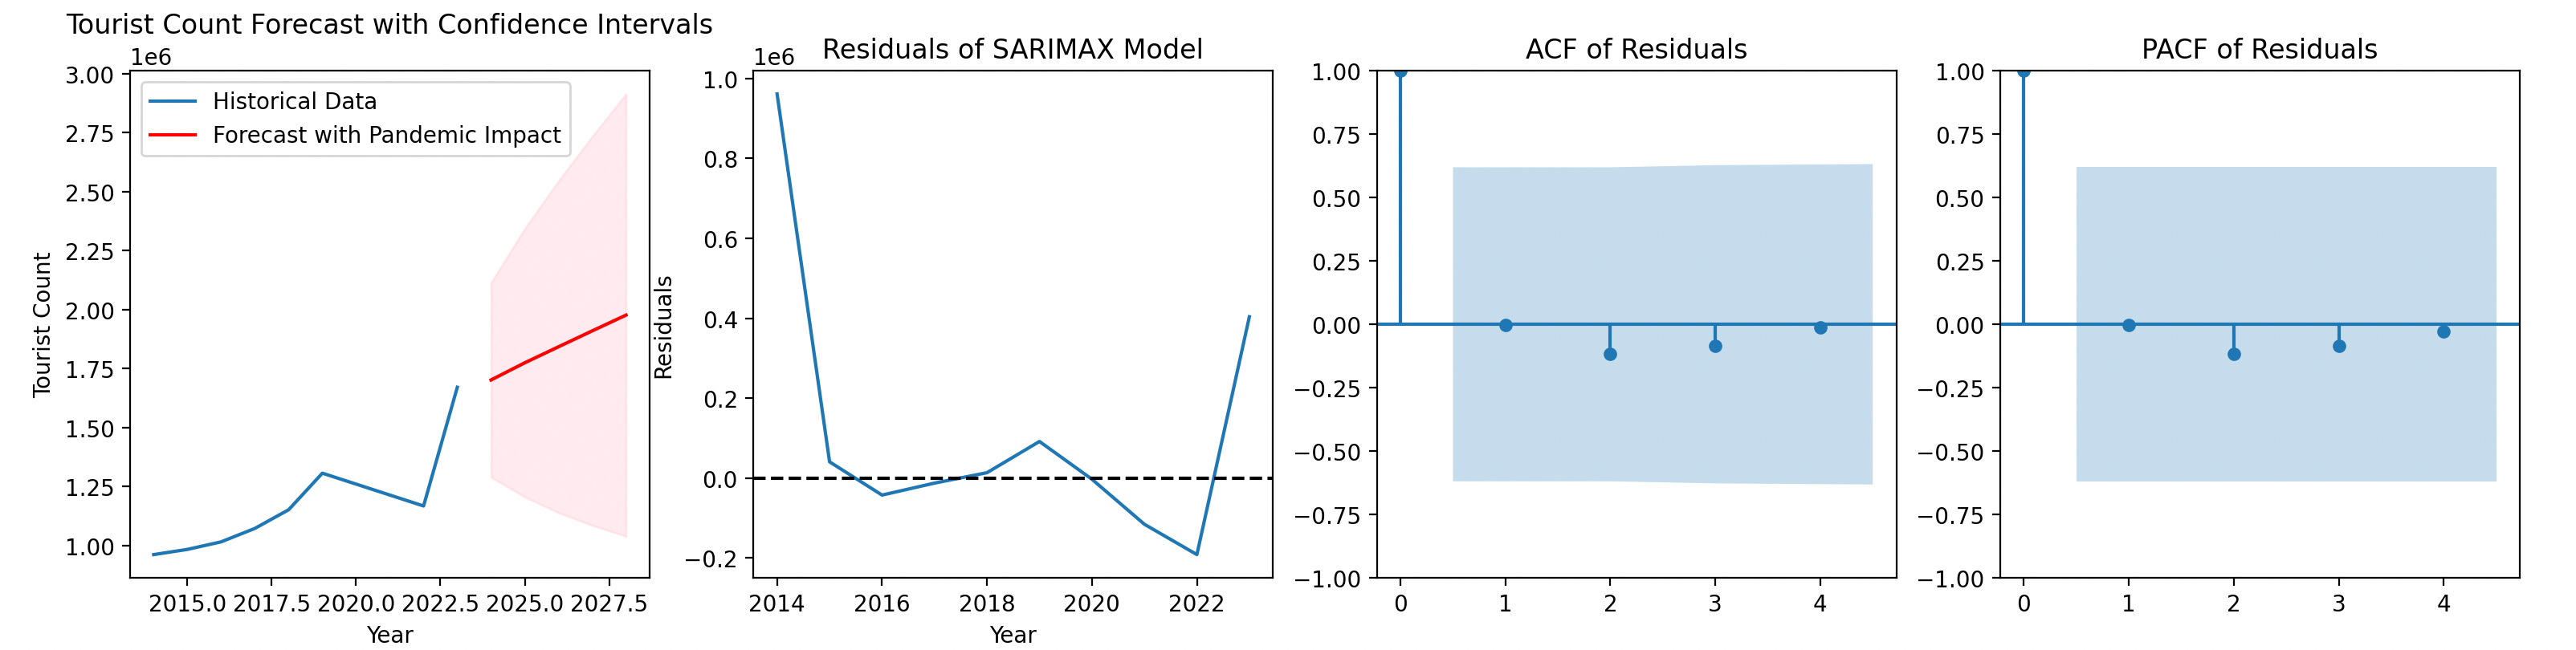
\includegraphics[width=1\textwidth]{Fig_Tourists.jpg} % 插入图片
    \vspace{-0.4cm}
    \caption{Tourist Prediction}
\end{figure}

It can be seen that the model correctly handles the plummet during the pandemic and
captures the trend of the revival of tourism. The exact number of 
tourists in the next few years is shown below, which will be utilized in the following sections.

\begin{table}[H]
    \centering
    \caption{Number of Tourists Prediction}
    \renewcommand{\arraystretch}{1.3}
 \begin{tabular}{|c|c|c|c|c|c|}
    \hline \textit{Year} & 2024 & 2025 & 2026 & 2027 & 2028 \\
    \hline \begin{tabular}{l} 
    \textit{Num(in thousands)} 
    \end{tabular} & 1701 & 1774 & 1842 & 1909 & 1976 \\
    \hline
    \end{tabular}
\end{table}



\subsection{Number of Local Residents}

\subsubsection{Population of Juneau}

According to \textit{World Population Review}, the population of Juneau in the last decade is as follows:

\begin{table}[H]
    \centering
    \caption{Population of Juneau}
    \renewcommand{\arraystretch}{1.3}
    \resizebox{\textwidth}{!}{
    \begin{tabular}{|c|c|c|c|c|c|c|c|c|c|c|c|c|c|c|c|}
        \hline \textit{Year} & 2010 & 2011 & 2012 & 2013 & 2014 & 2015 & 2016 & 2017 & 2018 & 2019 & 2020 & 2021 & 2022 & 2023 & 2024 \\
        \hline \textit{Num (in thousands)} & 31.4 & 32.2 & 32.4 & 32.6 & 32.5 & 32.6 & 32.5 & 32.1 & 32.0 & 32.0 & 32.2 & 32.0 & 31.7 & 31.6 & 31.3 \\
        \hline
    \end{tabular}
    }
\end{table}

\subsubsection{Population Prediction}

We still use the \textit{SARIMAX} model proposed in the last section
to predict the population of Juneau in the next few years. Parameters are the same as the last section.
The first four pictures are still the original data and predicted data, the residual, ACF and PACF plots.
In addition, official prediction data can also be found in \textit{World Population Review}, therefore two additional pictures are added to compare the prediction results.

\begin{figure}[H]
    \centering
    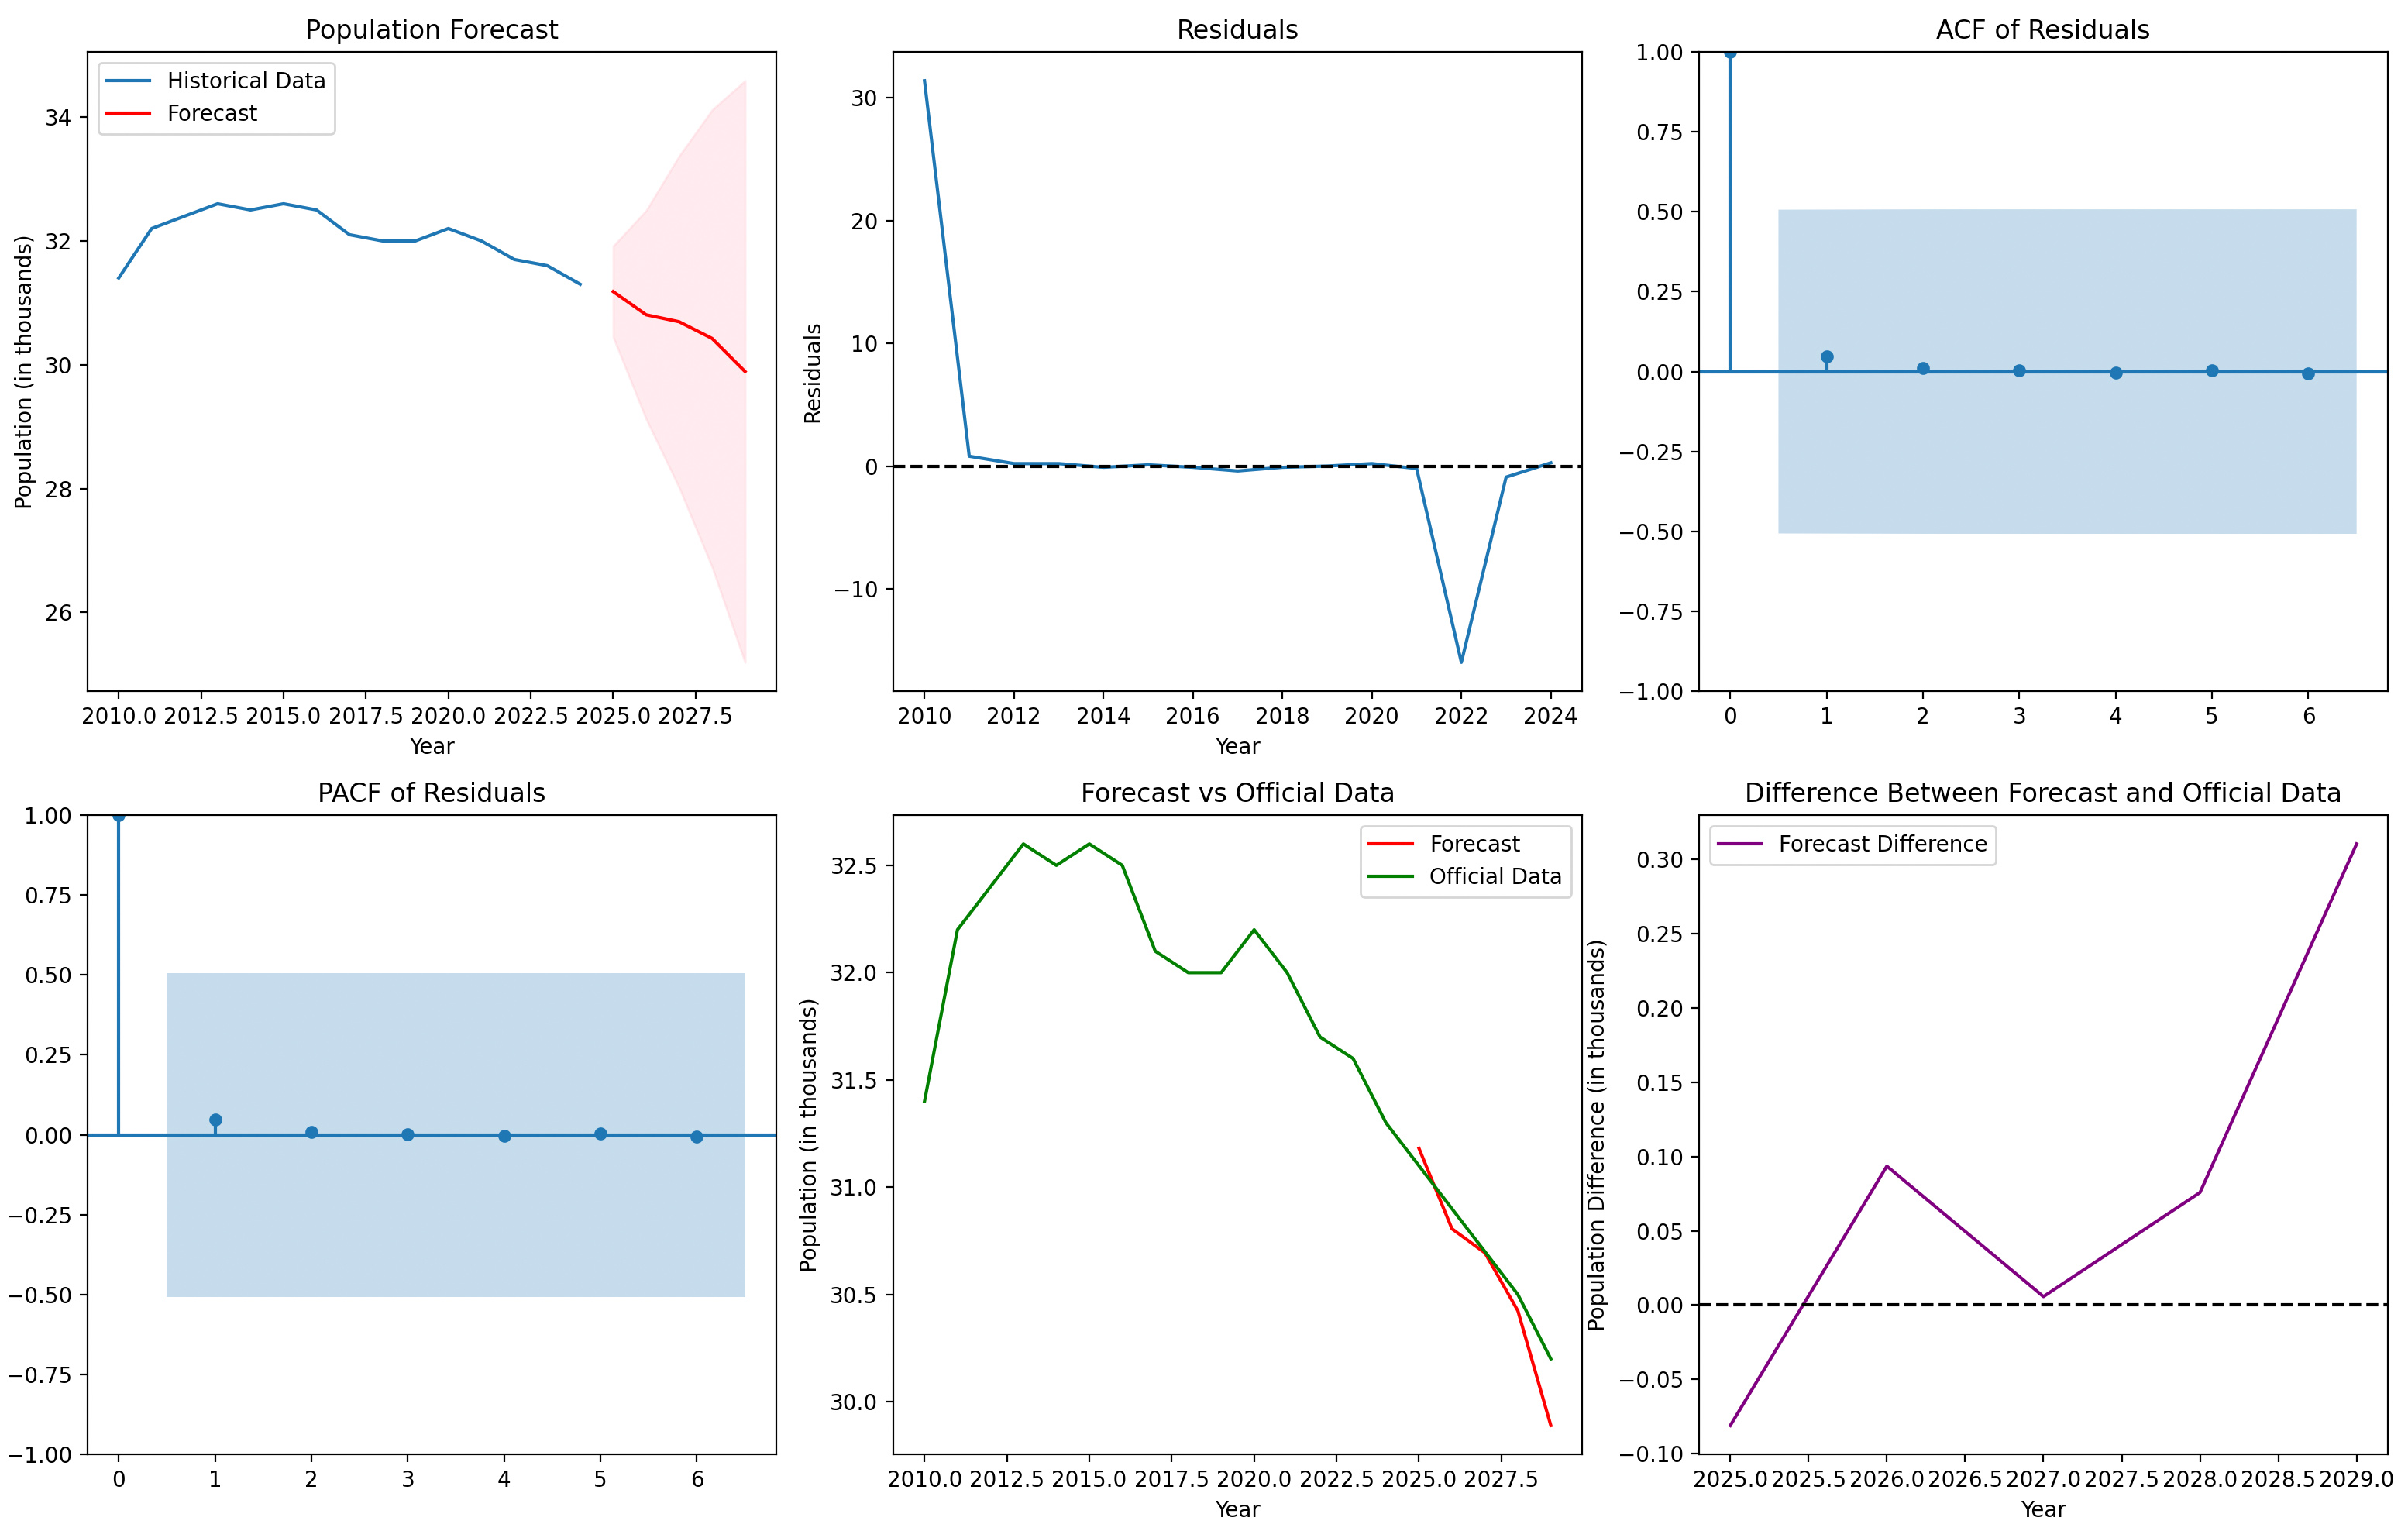
\includegraphics[width=1\textwidth]{Fig_Population.jpg} % 插入图片
    \vspace{-0.4cm}
    \caption{Tourist Prediction}
\end{figure}

It can be concluded from subfigure 5 and 6 that the model fits the data well 
and the prediction is reliable. The exact number of local residents in the next 
few years is shown below.

\begin{table}[H]
    \centering
    \caption{Population Prediction}
    \renewcommand{\arraystretch}{1.3}
 \begin{tabular}{|c|c|c|c|c|c|}
    \hline \textit{Year}  & 2025 & 2026 & 2027 & 2028 & 2029\\
    \hline \begin{tabular}{l} 
    \textit{Num(in thousands)} 
    \end{tabular} & 31.2 & 30.8 & 30.7 & 30.4 & 30.0 \\
    \hline
    \end{tabular}
\end{table}